% This LaTeX document needs to be compiled with XeLaTeX.
\documentclass[10pt]{article}
\usepackage[utf8]{inputenc}
\usepackage{ucharclasses}
\usepackage{graphicx}
\usepackage[export]{adjustbox}
\graphicspath{ {./images/} }
\usepackage{amsmath}
\usepackage{amsfonts}
\usepackage{amssymb}
\usepackage[version=4]{mhchem}
\usepackage{stmaryrd}
\usepackage{polyglossia}
\usepackage{fontspec}
\setmainlanguage{polish}
\setotherlanguages{thai}
\newfontfamily\thaifont{Noto Serif Thai}
\newfontfamily\lgcfont{CMU Serif}
\setDefaultTransitions{\lgcfont}{}
\setTransitionsFor{Thai}{\thaifont}{\lgcfont}

\title{50 ฉ }

\author{LIGA MATEMATYCZNA im. Zdzisława Matuskiego PÓŁFINAŁ 26 lutego 2019 SZKOŁA PODSTAWOWA\\
(klasy IV - VI)}
\date{}


\begin{document}
\maketitle
\begin{center}

\includegraphics[max width=\textwidth]{2024_11_21_71e9dc1a1f07adbf8fc8g-1}
\end{center}



\section*{ZADANIE 1.}
W pojedynczym ruchu można albo wrzucić do urny jedną kulkę, albo podwoić liczbę kulek znajdujących się w urnie. Wyznacz najmniejszą liczbę ruchów pozwalającą zamienić pustą urnę w urnę zawierającą 200 kulek.

\section*{ZADANIE 2.}
Bartek, jego ojciec i każdy z dwóch braci: Darek i Czarek obchodzą urodziny w lutym. Wiadomo, że mnożąc liczby lat obu braci Bartka otrzymujemy wiek Bartka, a mnożąc liczby lat całej trójki rodzeństwa dostajemy wiek taty. Ile lat ma tata Bartka, jeżeli wiadomo, że ma mniej niż 50 lat i każde z jego dzieci jest w innym wieku?

\section*{ZADANIE 3.}
Ile jest liczb trzycyfrowych podzielnych przez 9, które można ułożyć z cyfr 2, 7, 9, 0 wykorzystując w jednej liczbie każdą z cyfr co najwyżej raz? Podaj wszystkie możliwości.

\section*{ZADANIE 4.}
W równoległoboku \(A B C D\) bok \(A B\) jest dwa razy dłuższy od boku \(B C\). Punkt \(M\), dzielący bok \(A B\) na połowy, połączono z punktami \(C\) i \(D\). Oblicz miarę kąta \(C M D\).

\section*{ZADANIE 5.}
Obwód pięciokąta wypukłego \(A B C D E\) jest równy 74 , obwód czworokąta \(A B C D\) jest równy 56, a czworokąta \(A C D E-37\). Oblicz obwód trójkąta \(A C D\).\\
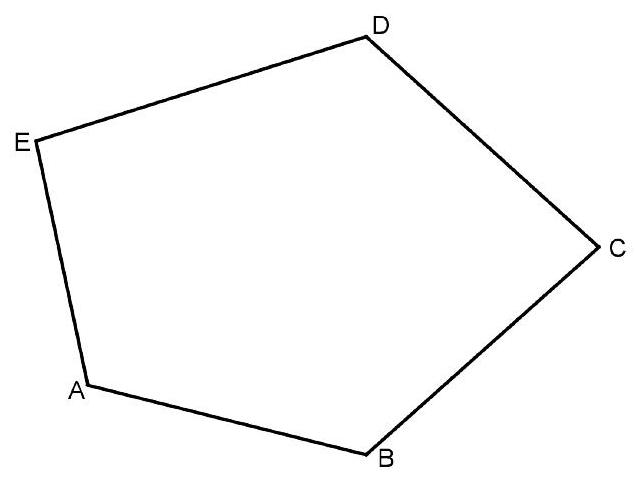
\includegraphics[max width=\textwidth, center]{2024_11_21_71e9dc1a1f07adbf8fc8g-1(1)}


\end{document}